\subsection{Gravitational acceleration inside the Earth}
Knowing the gravitational acceleration \textit{inside} the Earth is important, e.g., for understanding processes related to mantel convection.
\begin{enumerate}[label=(\alph*)]
  \item Use the consequences of the shell theorem to predict the gravitational acceleration $g(r)$ inside a spherical Earth. First assume that the Earth's density is constant, then that it decreases linearly with distance from the center. Assume that the density in the core is approximately $\rho_{core} = 13 \frac{g}{cm^3}$ and in the crust approximately $\rho_{crust} = 2.7 \frac{g}{cm^3}$.

  \item Draw the results on a x-y graph on paper or using a software of your choice.

  \item The PREM model (Fig. \ref{Fig:PREM})provides an observationally constrained estimate of the density distribution inside the Earth. Knowing the shape of this profile, what is your guess of the gravitational acceleration inside the Earth? Why is it more difficult for you to calculate this quantitatively compared to the previous cases of constant and linearly varying density?

  \item Extra: Calculate the gravitational acceleration inside the Earth based on the PREM model using Matlab/Python/Excel. The data can be found on Ilias.
\end{enumerate}

\begin{figure}
    \label{Fig:PREM}
    \begin{center}
    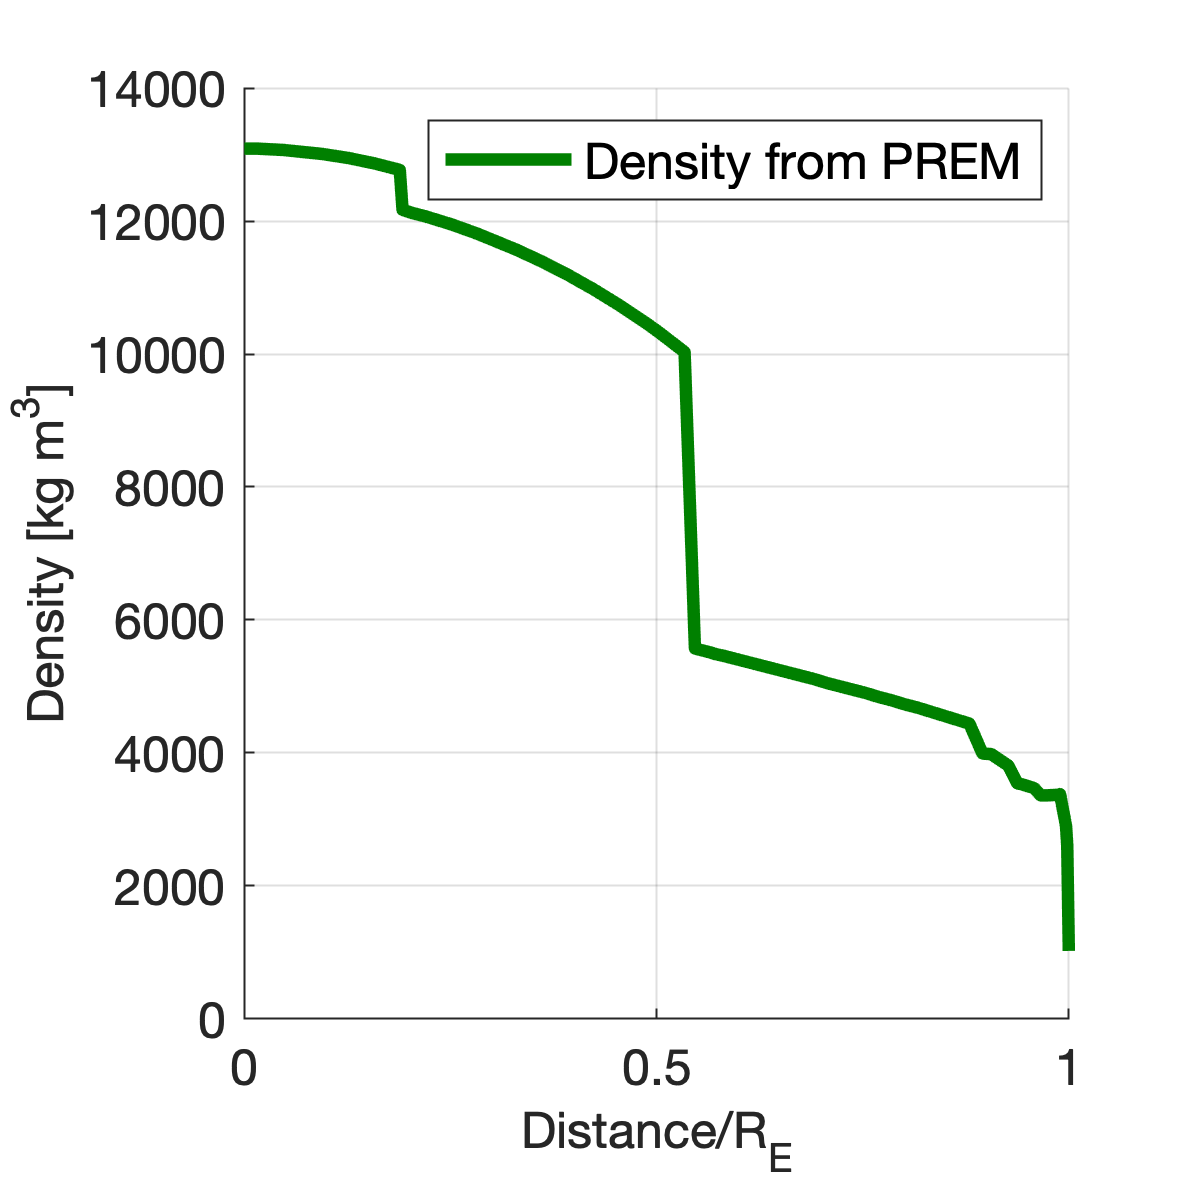
\includegraphics[width=0.5\textwidth]{Figures/Gravimetry/Gravimetry01_PREM.png}
    \caption{The Preliminary Reference Earth Mode (Dziewonski, A. M. \& Anderson, D. L, 1981).}
    \end{center}
\end{figure}
\ifanswers
    \begin{tcolorbox}[enhanced jigsaw,breakable,pad at break*=1mm,
    colback=blue!5!white,colframe=babyblueeyes,title=Solutions,
    watermark color=white]
 
      (a) At location $l<R$ inside the Earth, we do not need to worry about the mass distribution for distances $>l>R$ as these will cancel out due to the spherical symetry. Also the the acceleration will only have a radial component. Hence,
    \begin{equation}
        |\vec{g}(l)| = G\frac{M}{l^2}
    \end{equation}
    where $M$ is mass contained in the sphere with radius $l$. How does $M$ change as we change $l$? In this spherical symetry it is best to adopt spherical coordinates so that we can write: 
    \begin{eqnarray}
    M &=& \int \rho dV \\ 
    &=& \int_0^{\pi} d\theta \sin(\theta) \int_0^{2\pi}  d\phi \int_0^l dl\,\rho\,l^2 dV
    \end{eqnarray}
    this is a fairly complicated way of writing something that you know by heart (i.e. the density times the volume of a sphere), but this is a good oppertunity to make use of spherical coordinates. Most importantly, it is worthwhile to remember that the volume element $dV = l^2 \sin(\theta)drd\theta d\phi$ is quite different from the cartesian coordinates that you are used to otherwise. Also take a moment and understand why the integration limits are the way they are. Solving the integral step by step for the case of a constant density:
    \begin{eqnarray}
        M &=& \rho \int_0^{\pi} d\theta \sin(\theta)\int_0^{2\pi}  d\phi \int_0^l l^2 dl \\
         &=&\rho 2\pi \int_0^{\pi} d\theta \sin(\theta)\int_0^l l^2dl\\
         &=&\rho 4\pi \int_0^l l^2dl \\ 
         &=&\rho \frac{4}{3}\pi l^3
    \end{eqnarray}
    Plugging (7) into (1) then results for $l<R$:
    \begin{equation}
        |\vec{g}(l)| = G  \rho \frac{4}{3}\pi \frac{l^3}{l^2} = G  \rho \frac{4}{3}\pi l
    \end{equation}
    so the gravitational acceleration increases linearly with distance from the Earth's center as long as $l<R$ and $\rho$ is constant. A linear decrease of density with increasing distance can be parameterized as:
    \begin{equation}
        \rho(l) = \frac{\rho_{crust}-\rho_{core}}{R} (l-R) + \rho_{crust} = \frac{\rho_{crust} - \rho_{core}}{R}l+\rho_{core}
    \end{equation}
    As the density now changes with $l$ we cannot take it out of the integration. In particular for eq. (6) this means:
    \begin{eqnarray}
        M &=& 4\pi \int_0^l dl \left(\frac{\rho_{crust} - \rho_{core}}{R}l^3+\rho_{core}l^2\right)\\
          &=& 4\pi \left(\frac{\rho_{crust} - \rho_{core}}{4R}l^4+\frac{1}{3}\rho_{core}l^3 \right)
    \end{eqnarray}
    so that:
    \begin{eqnarray}
        |\vec{g}(l)| &=& 4 G \pi \frac{1}{l^2} \left(\frac{\rho_{crust} - \rho_{core}}{4R}l^4+\frac{1}{3}\rho_{core}l^3 \right) \\
        &=& 4 G \pi \left(\frac{\rho_{crust} - \rho_{core}}{4R}l^2+\frac{1}{3}\rho_{core}l \right)
    \end{eqnarray}
    \begin{center}
        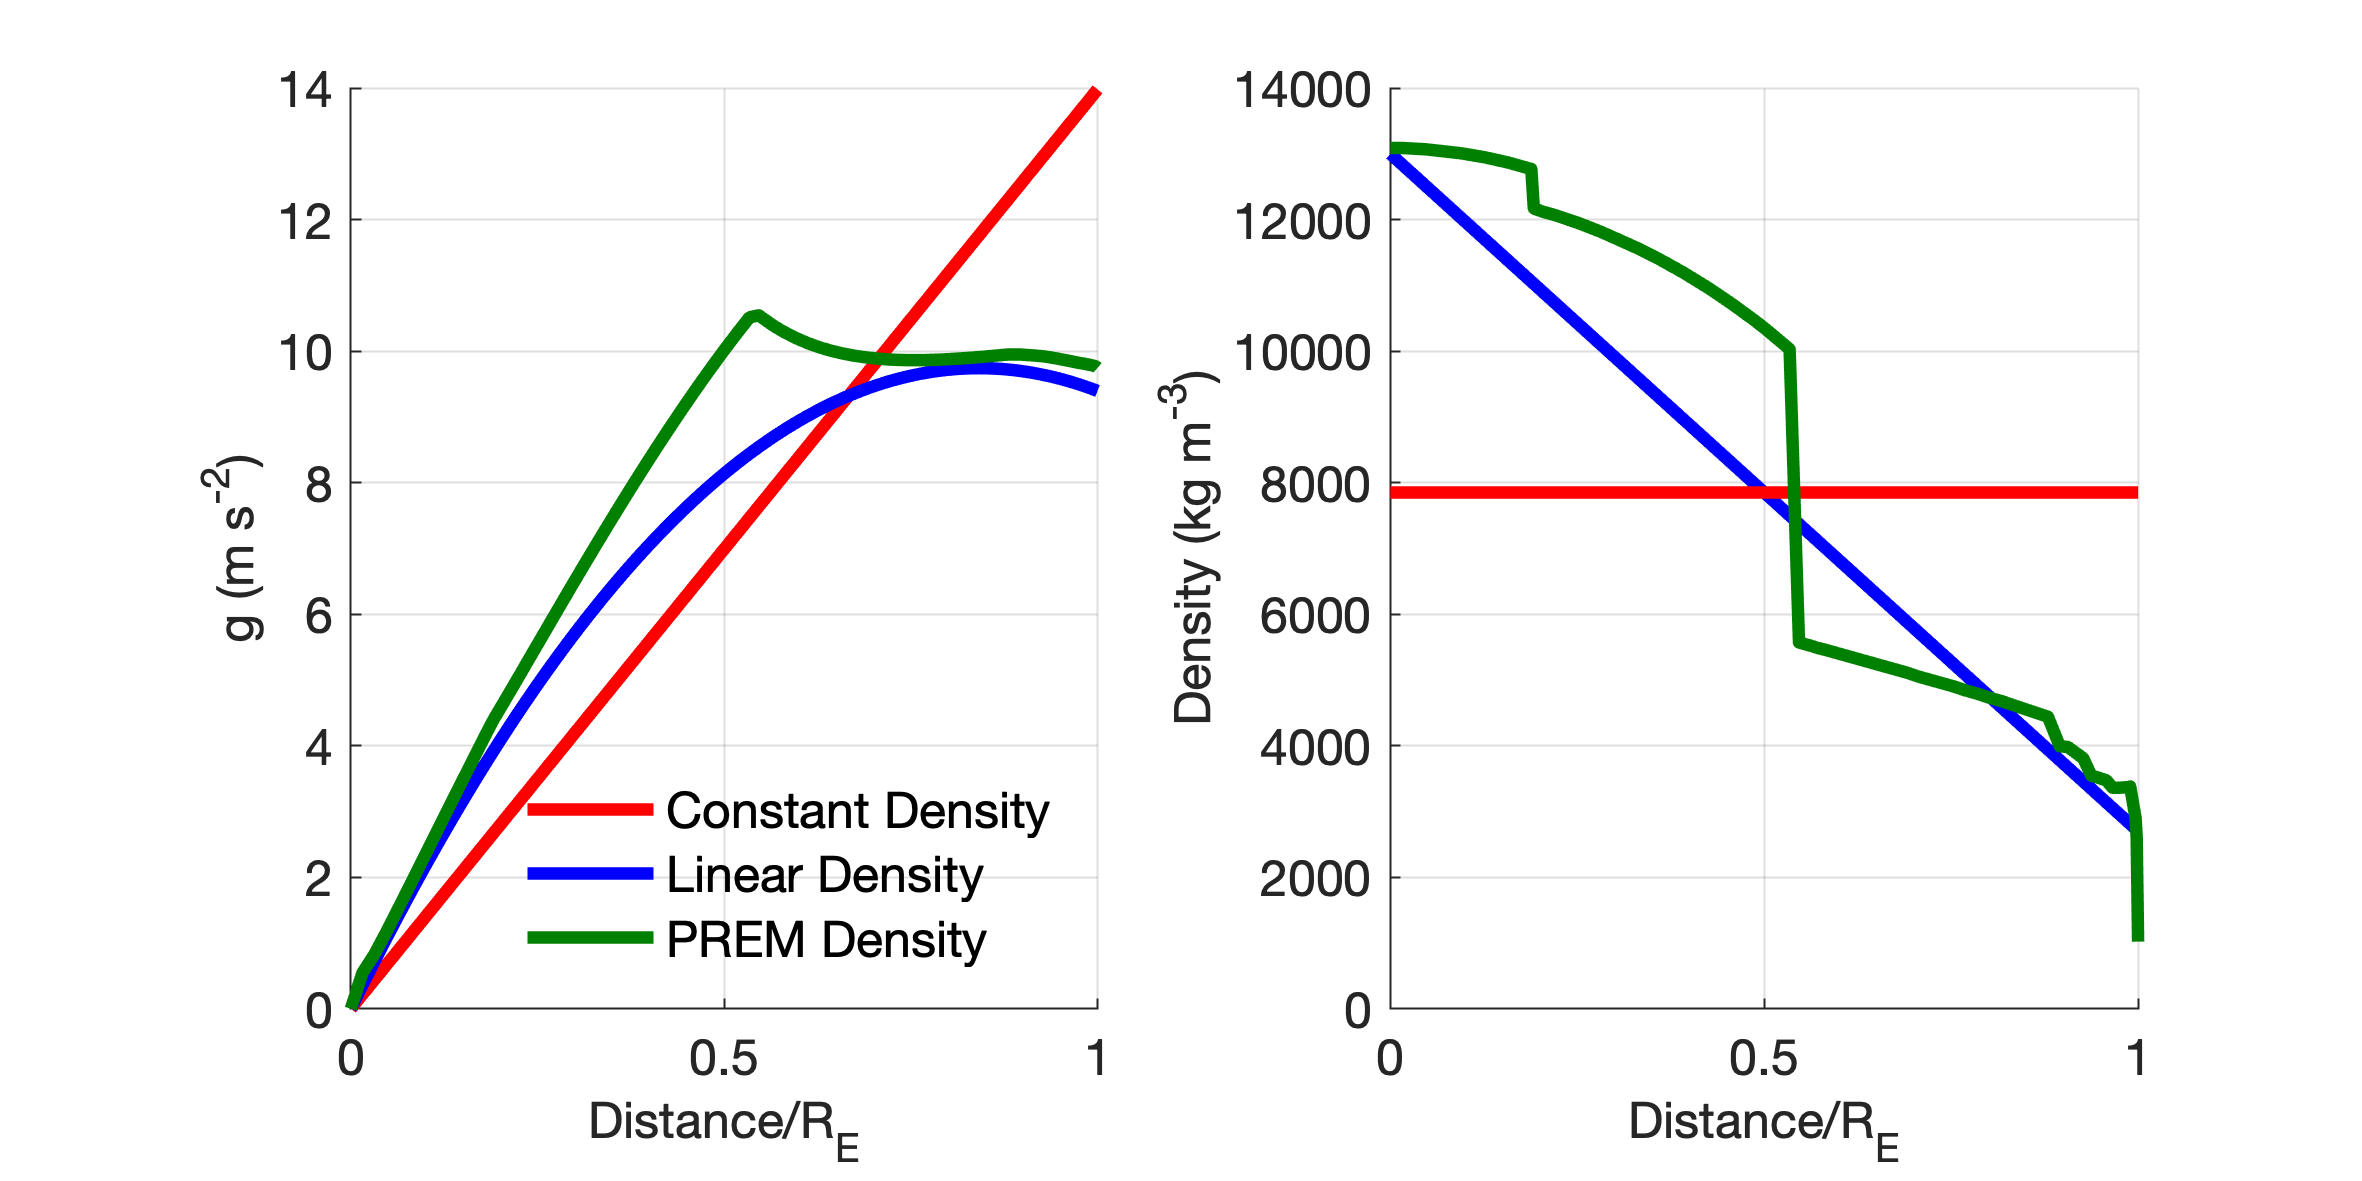
\includegraphics[width=0.99\textwidth]{Figures/Gravimetry/Gravimetry01_GravityInsideEarth.png}
     \end{center}
     so that the gravitational acceleration now changes quadratically as shown in the Figure above. Is this realistic? We will have to compare it with a realistic dataset such as the PREM model.

  (c) Because we don't have an analytical expression for the PREM density model, we cannot pursue an analytical integration as done in the previous two cases. Hence we do it numerically:
     \lstinputlisting[language=matlab]{../../Src/Exercises/Gravimetry/Gravimetry03_GravityInsideSphere.m}
    \end{tcolorbox}
\fi